\documentclass{article}%
\usepackage[T1]{fontenc}%
\usepackage[utf8]{inputenc}%
\usepackage{lmodern}%
\usepackage{textcomp}%
\usepackage{lastpage}%
\usepackage[head=40pt,margin=0.5in,bottom=0.6in]{geometry}%
\usepackage{graphicx}%
%
\title{\textbf{Rechazan incluir Venezuela entre "países terroristas"}}%
\author{Diario El Universal}%
\date{23/11/2018}%
%
\begin{document}%
\normalsize%
\maketitle%
\textbf{URL: }%
http://www.eluniversal.com/politica/26495/rechazan{-}incluir{-}venezuela{-}entre{-}paises{-}terroristas\newline%
%
\textbf{Periodico: }%
EU, %
ID: %
26495, %
Seccion: %
politica\newline%
%
\textbf{Palabras Claves: }%
NO\_TIENE\newline%
%
\textbf{Derecho: }%
CONTEXTO%
, Otros Derechos: %
NO\_TIENE%
, Sub Derechos: %
NO\_TIENE%
\newline%
%
\textbf{EP: }%
NO\newline%
\newline%
%
\textbf{\textit{Líder del partido Demócrata señala que Trump tendría que demostrarlo}}%
\newline%
\newline%
%
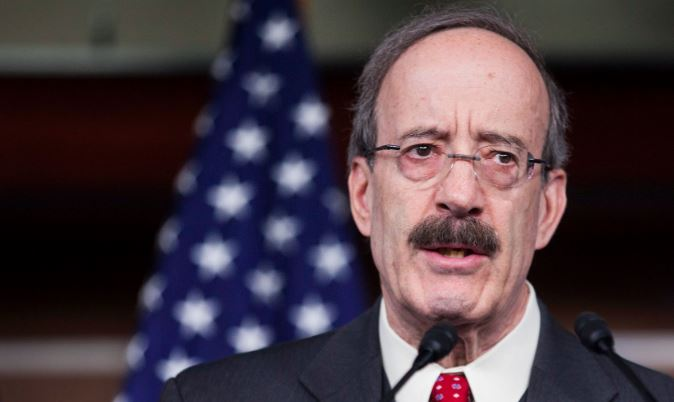
\includegraphics[width=300px]{126.JPG}%
\newline%
%
Miembros del partido demócrata de Estados Unidos cuestionaron ayer la posibilidad de incluir a  Venezuela en la lista del gobierno estadounidense de "países que promueven y  financian el terrorismo".%
\newline%
%
El rechazo surge de una versión periodística de The Washington Post, según la cual "la administración del presidente Donald Trump se está preparando para agregar a Venezuela a la lista de países señalados como patrocinadores del terrorismo lo que podría volverse una dramática escalada contra el Gobierno del presidente Nicolás Maduro".%
\newline%
%
La presunta decisión de incluir a Venezuela en la citada lista, ha sido propiciada por el senador republicano Marco Rubio, quien ha escrito al presidente y al secretario de Estado, Mike Pompeo, relatando las relaciones del chavismo con grupos terroristas como la banda vasca ETA, la milicia chií Hezbolá y la guerrilla colombiana de las FARC, según la información del The Washington Post.%
\newline%
%
Reseñan por su parte agencias de noticias, que el líder de la minoría demócrata en la Cámara, Eliot Engel, expresó que "si Donald Trump decide añadir al Estado venezolano en el listado que incluye a Corea del Norte, Irán, Sudán y Siria "debe demostrar que Caracas ha apoyado de forma repetida actos de terrorismo internacional".%
\newline%
%
Engel expresó que, de momento no ha visto pruebas de que el gobierno venezolano se encuentre involucrado en ese tipo de actos, para ser incluido en la mencionada lista de países terroristas, pese a que admite que el presidente Maduro "viola los derechos de los ciudadanos  a diario".%
\newline%
%
\end{document}